% TODO outline how multiple applications share the ecoviser/api

Figure \ref{fig:system_design} illustrates our general system design approach
that simulates the ecovisor infrastructure and integrates it into the Mosaik
co-simulation environment while enabling SIL capabilities. The present design
can be categorized into two distinct parts, the simulation of the ecovisor, and
its interface to external applications, which are elaborated on in the
following.

\begin{figure}
    \centering
    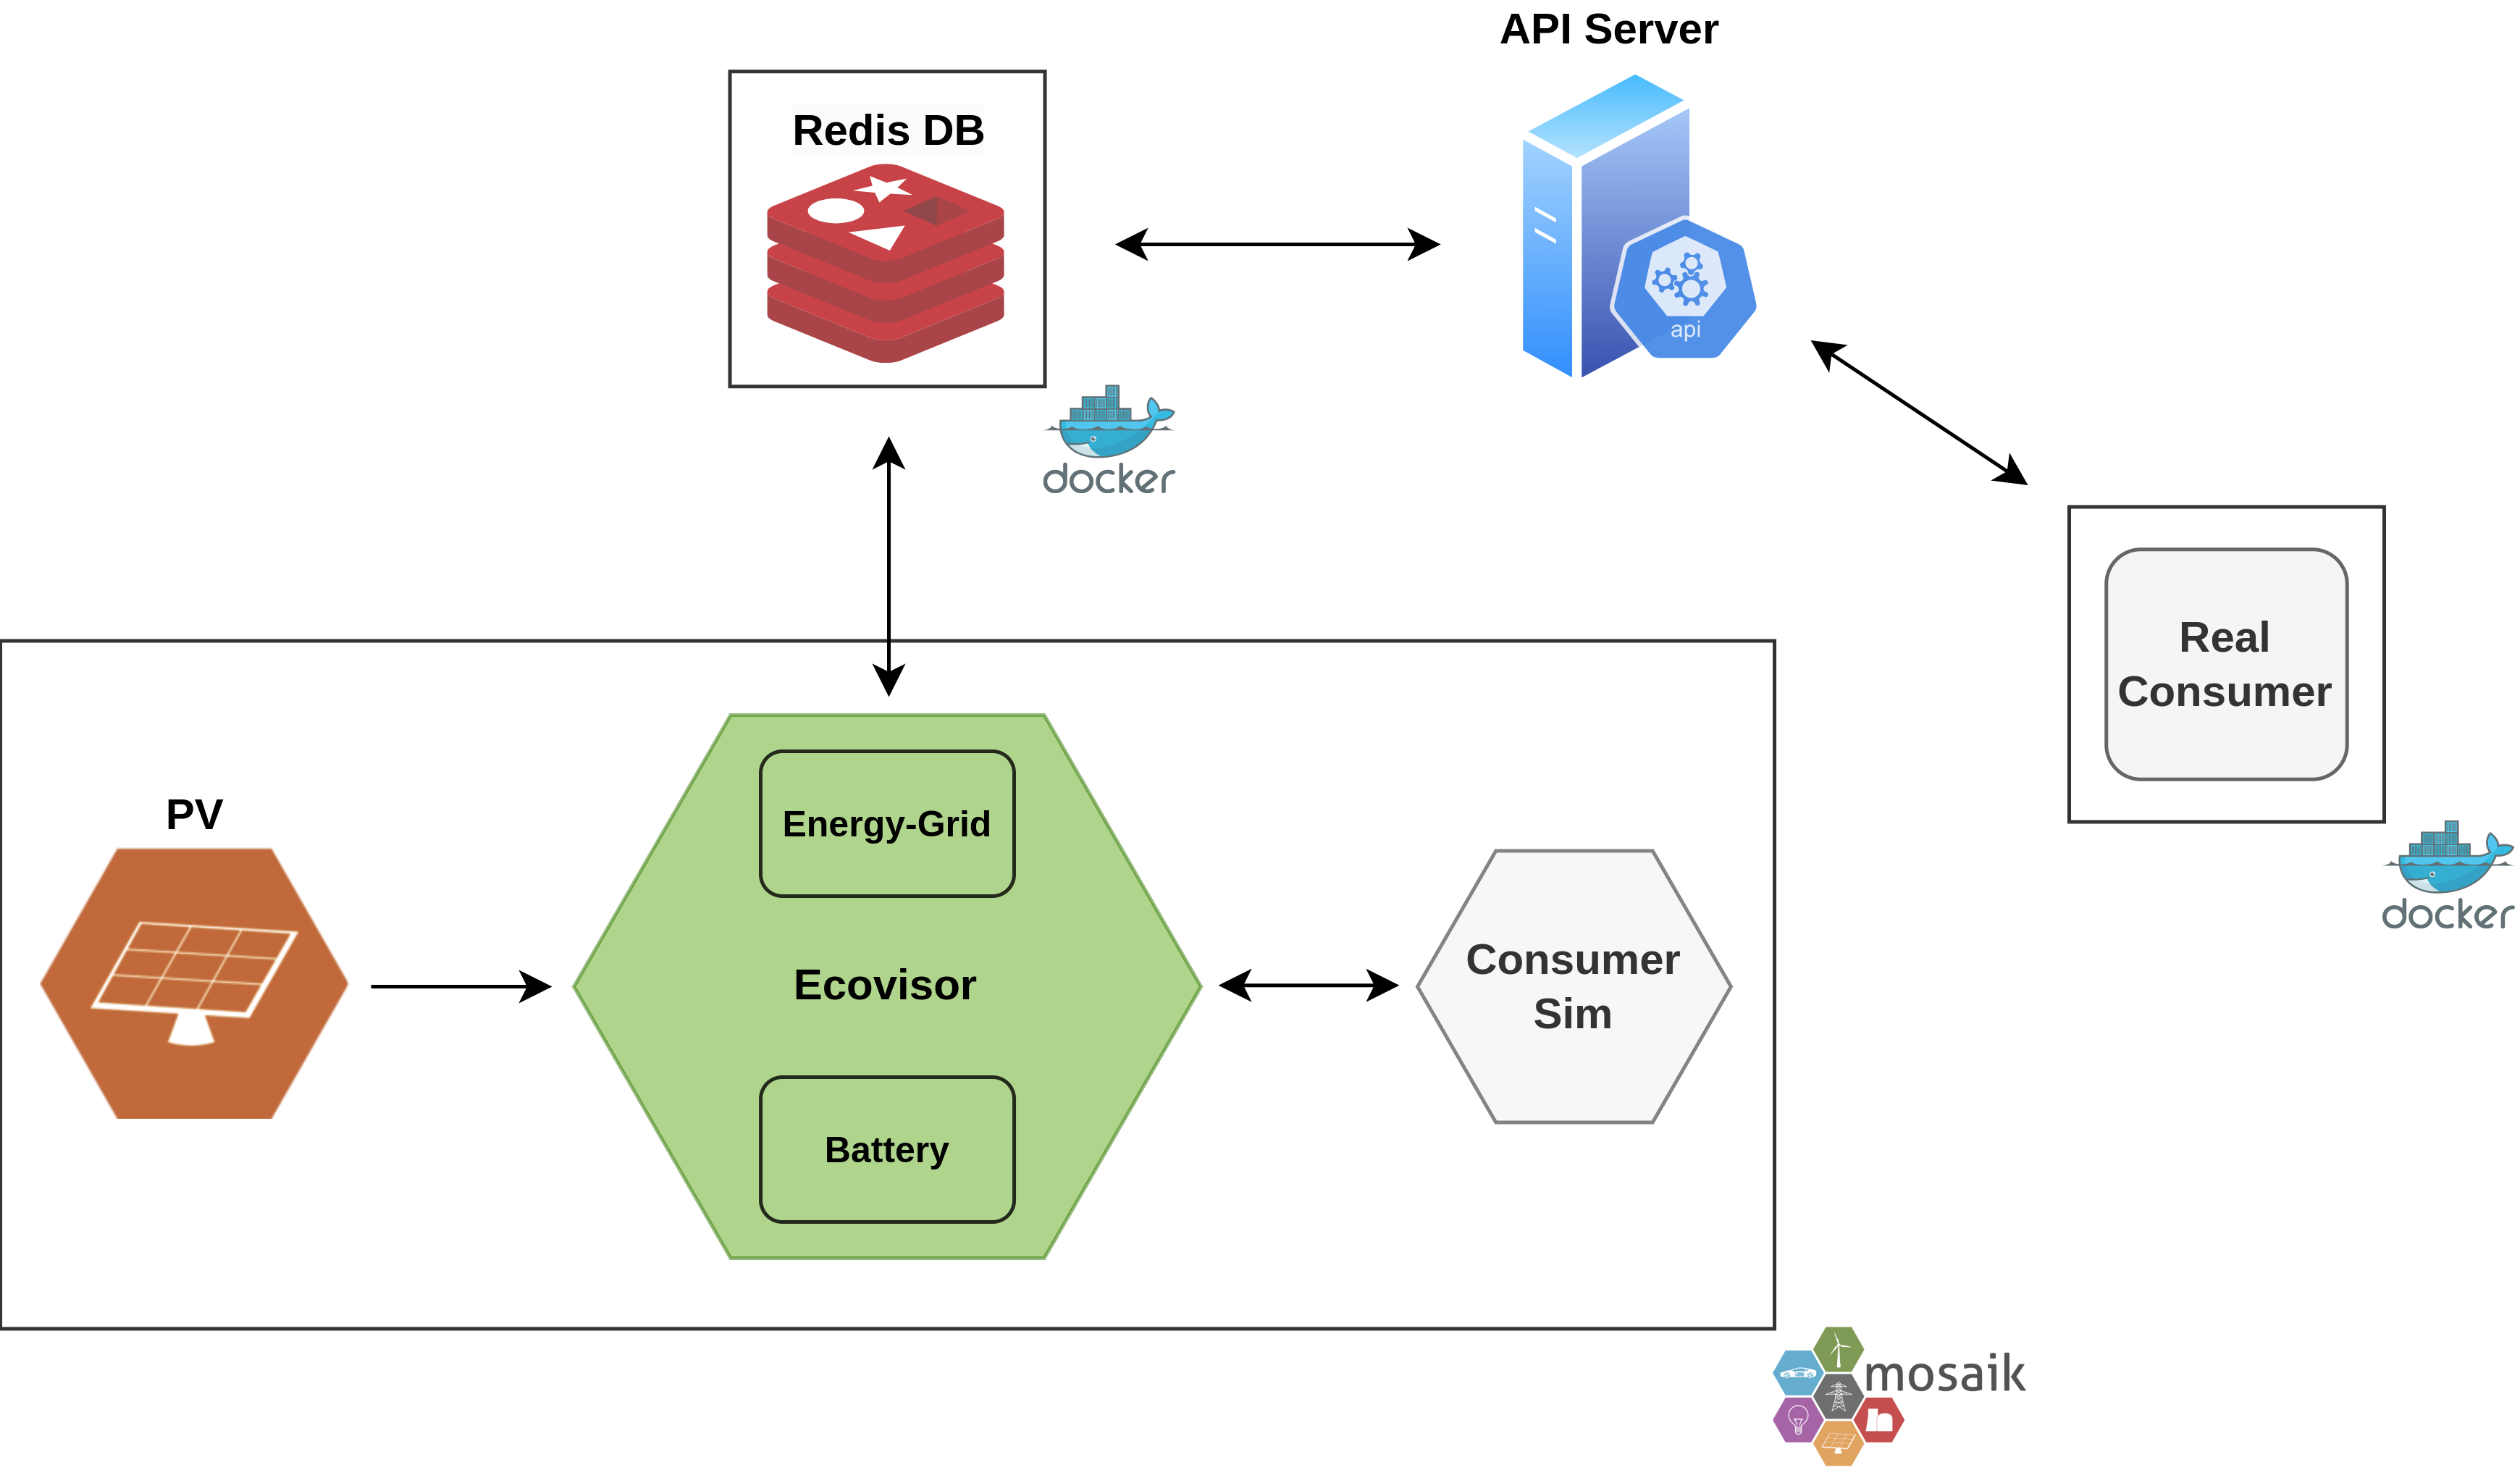
\includegraphics[width=\linewidth]{figures/system_design}
    \caption{
        General System Design: The ecovisor infrastructure is simulated and
        integrated into the Mosaik co-simulation environment. SIL capabilities
        are enabled via an API Server and a Redis database, connecting the
        simulation environment and real applications in real-time.
    }
    \label{fig:system_design}
\end{figure}

\subsection{Simulation of the Ecovisor}
% sim consists of multiple components, namely the ecoviser itself, pv sim and
% agent, consumer sim and agent, explain what they do
%
% explain how the model in integrated in mosaik -> api, methods and what they do
% maybe to background?
%
% explain the virtual_energy_system_simulation with code
%
% sim runs in real time -> rt_factor=1
% https://mosaik.readthedocs.io/en/latest/scenario-definition.html?highlight=real%20time#how-to-do-real-time-simulations
%
% all models are time-based and 1 step = 1 second -> power is modeled in kWs
%
% monitoring through agent (maybe explain agent in background?)

The simulation part of our approach is fully contained within the Mosaik
co-simulation environment. In Figure \ref{fig:system_design} this includes the
photo-voltaic (PV) module, the ecovisor and a consumer simulator. The consumer
and PV module simulators utilized in this context are the \texttt{mosaik-csv}
simulator, which is a component of the Mosaik ecosystem \cite{mosaik_ecosystem}.
This simulator is capable of simulating CSV datasets, and in the current
application, it is employed to simulate consumption data and recorded or
forecasted PV data. While our primary focus is to facilitate the integration of
external, non-simulated applications with our simulated ecovisor, we also
recognize the need to accommodate simulated consumers for more sophisticated
approaches that require additional data. Therefore, we aim to provide
flexibility in our system to meet a wide range of requirements. Because these
two components are designed to be minimal and replaceable, they each require a
controller agent that acts as a medium between the component and the simulated
ecovisor. The controller can be initialized with e.g. a power conversion factor
to allow for the use of different measurement units in the datasets, as the
standard power unit utilized in the ecovisor is kW.

%The simulated ecovisor is abstracted from the original design. Our approach does
%not implement a COP/Hypervisor. We


% TODO comment code a bit
\begin{figure}
    \removelatexerror
    \begin{algorithm}[H]
        \caption{Virtual Energy System Simulation}
        \label{alg:virtual_energy_system_simulation}
        $rest \gets consumption - solar$\;
        \eIf{$rest \leq 0$} {
            $b\_discharge\_rate \gets 0$\;
        }{
            $b\_discharge\_rate \gets \text{min}($\;
            \Indp
                $b\_max\_discharge,$\;
                $b\_charge\_level \cdot 3600,$\;
                $rest$\;
            \Indm
            $)$\;
            $rest \gets rest - b\_discharge\_rate$\;
        }
        $grid\_power \gets b\_charge\_rate + rest$\;
        $b.delta \gets b\_charge\_rate - b\_discharge\_rate$\;
        $b.step()$\;
        $b\_charge\_level \gets b.charge$\;
        $total\_carbon \gets grid\_carbon \cdot grid\_power$\;
        \vspace{3mm}
    \end{algorithm}
\end{figure}

\subsection{Interface to External Applications}
%TODO: Second itteration on writing

To connect the Ecovisor-Model to a real workload-application, we exposed the API which is described in \cite{souza2023} to containerized workloads.we have tried to implement it in a way that is as close as possible to a real implementation in a cloud environment.
To achieve that, we implemented the Ecovisor-API from \cite{souza2023}, which can be seen in \ref{table:ecovisor_api}, into an FastAPI server \cite{fastapi}. %TODO fußnote oder quelle?
The API-Server is connected to a RedisDB\cite{redis}, which serves as a key-value store and links the API-Server to the Ecovisor-Model. 
The Ecovisor-Model itself implements an Redis-Interface to read and write data from the RedisDB.
In the following three sections we will describe these three parts of the \textit{External Application Interface} in depth.
%TODO Gründe für den arch ansatz

\subsubsection{API-Server} %TODO kein tick
The API-Server exposes the Ecovisor-API to the "Workloads". It is implemented with the FastAPI Framework and utilizes the Uvicorn Web-Server \cite{uvicorn} to handle multiple clients accessing the API. Due to the ASGI (Asynchronous Server Gateway Interface) nature of the Web-Server, the module is started as a independent thread. The advantage of this, is that the server can handle multiple clients, which will be useful when multiple workloads will be connected to the simulation. On the other hand, the implementation into the system is more difficult, so that we decided to start the module independently. In earlier versions we tried to implement it inside of the Ecovisor-Model, but it would stops the execution of the simulation until the API-Server is stopped which renders the system unusable. This also enables the API-Server to be scaled independent from the Ecovisor-Model and the RedisDB. This may be helpful in bigger simulations with distributed infrastructure.

\subsubsection{RedisDB}
The RedisDB is a fast, in memory, key-value store for simple data-types. In our system, it is used to save and provide the data from within the Ecovisor-Model to the API-Server. To keep the operability of the simulation simple, the RedisDB is started as a Docker Container via the docker python library \cite{docker_python}, which implements the docker engine API into python. The container image we used is the redislabs rejson redis image \cite{RedisJSON}. This images extends the RedisDB image with the capability to process JSON values. The Redis-Container is started right at the beginng of the simulation, so that it is up and operational when the first data is available. After the end of the simulation, the container is stopped and deleted to keep the test environment free of remnants of t he simulation. 
In general the database can easily be exchanged with any other database by adapting the Ecovisor-Redis-Interface in the Ecovisor-Model. This can be useful when simulation should be integrated
in a production grade cloud environment like kubernetes or openstack.


%Since the values are updated in one write atomicity is ensured, but due to the dataflow described in \ref{subsec:dataflow}
%atomicity isnot requierd to keep the values consistent.



%TODO values picture
%\begin{figure}
%    \centering
%    \includegraphics[width=\linewidth]{}
%    \caption{Datastructur of exchanged Data}
%    \label{fig:ecovisor_api}
%\end{figure}
\begin{figure}
	\removelatexerror
	\begin{algorithm}[H]
		\caption{Example Redis Data JSON}
		\label{alg:redis_JSON}
		\{\;
			$"solar\_power" : "0 kW",$\;
			$"grid\_power" : "0 kW",$\;
			$"grid\_carbon" : "0 g*CO2/kW",$\;
			$"battery\_discharge\_rate" : "0 kW",$\;
			$"battery\_charge\_level" : "0 kWh"$\;
		\}
		\vspace{3mm}
	\end{algorithm}
\end{figure}

\subsubsection{Ecovisor-Redis-Interface}
The interface from the ecovisor towards the redisdb is implemented within the ecovisor model. To simplify the usage, the redis python libary %source
is used. The ecovisor model implements two methods, the
\texttt{get\_redis\_updates()} and the \texttt{send\_redis\_updates} %TODO methoden mit code abgleicehn und formatieren

The \texttt{get\_redis\_update} method gets the values (...) as show in (ref) from the RedisDB %TODO insert valzes and reference to the
and writes it to the ecovisor model variables to make them usable for the ecovisor model.

the \texttt{send\_redis\_updates()} method publishes the updated values from the other part of the simulation which are accessible by the ecoviser shwon in (ref) model to the redisdb to make it
usable by the workload application. %TODO raus wegen dopplung?

In each step the ecovisor model first gets the updates from the RedisDB, processes the data and then sends the updated data to the RedisDB, to make it
acessible to the workload application.

%code?
\subsubsection{Dataflow}
\label{subsec:dataflow}
%TODO Picture Data-Flow (Values set by Ecovisor, Values set by Workload)
\begin{figure}
    \centering
    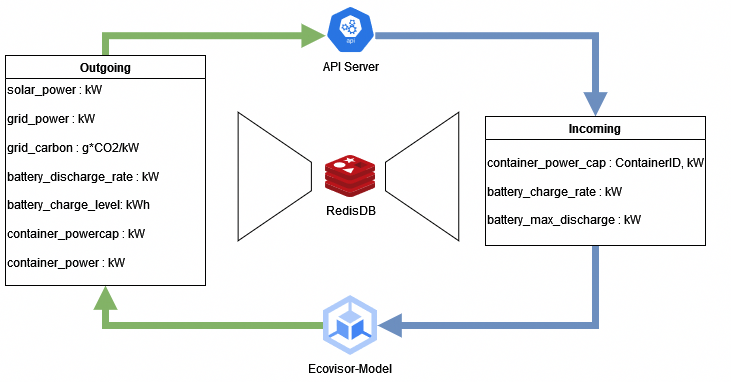
\includegraphics[width=\linewidth]{figures/Dataflow.drawio.png}
    \caption{Dataflow betwen Ecovisor-Model and API Server}
    \label{fig:dataflow}
\end{figure}

The Values/Data shown in (ref) is exchanged between the ecovisor model and the API server via the RedisDB. There are two main streams of the dataexchange.
First from the ecovisor model to the API-Server and second from the API-Server to the ecovisor model. There are no values which are used in both streams, which makes things
easier in terms of consistency and parallel access.

As stated before, the data is updated in each simulation step. (ref)
In the downstream, from the ecovisor to the API-Server the values (...) are updated and can be consumed by the workload applications
and in the upstream, from the api-server to the ecovisor model, the values (...) are updated and used by the ecovisor model to calculate (...) %abgleich mit code
%TODO referenz bild einbinden

